\section{eo\-Op\-Container$<$ EOT $>$ Class Template Reference}
\label{classeo_op_container}\index{eoOpContainer@{eoOpContainer}}
eo\-Op\-Container is a base class for the sequential and proportional selectors It takes care of wrapping the other operators, and deleting stuff that it has allocated  


{\tt \#include $<$eo\-Op\-Container.h$>$}

Inheritance diagram for eo\-Op\-Container$<$ EOT $>$::\begin{figure}[H]
\begin{center}
\leavevmode
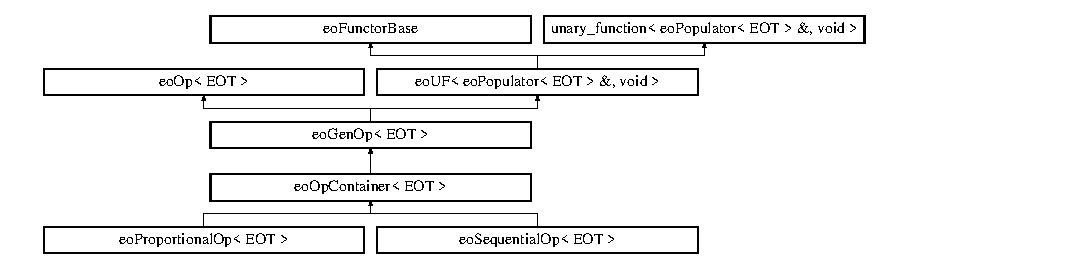
\includegraphics[height=3.18544cm]{classeo_op_container}
\end{center}
\end{figure}
\subsection*{Public Member Functions}
\begin{CompactItemize}
\item 
{\bf eo\-Op\-Container} ()\label{classeo_op_container_a0}

\begin{CompactList}\small\item\em Ctor: nothing much to do. \item\end{CompactList}\item 
virtual {\bf $\sim$eo\-Op\-Container} (void)\label{classeo_op_container_a1}

\begin{CompactList}\small\item\em Dtor: delete all the Gen\-Ops created when wrapping simple ops. \item\end{CompactList}\item 
virtual unsigned {\bf max\_\-production} (void)\label{classeo_op_container_a2}

\begin{CompactList}\small\item\em for memory management (doesn't have to be very precise \item\end{CompactList}\item 
void {\bf add} ({\bf eo\-Op}$<$ {\bf EOT} $>$ \&\_\-op, double \_\-rate)
\begin{CompactList}\small\item\em Add an operator to the container, also give it a rate. \item\end{CompactList}\item 
virtual std::string {\bf class\-Name} () const =0\label{classeo_op_container_a4}

\end{CompactItemize}
\subsection*{Protected Attributes}
\begin{CompactItemize}
\item 
std::vector$<$ double $>$ {\bf rates}\label{classeo_op_container_p0}

\item 
std::vector$<$ {\bf eo\-Gen\-Op}$<$ {\bf EOT} $>$ $\ast$ $>$ {\bf ops}\label{classeo_op_container_p1}

\end{CompactItemize}
\subsection*{Private Attributes}
\begin{CompactItemize}
\item 
{\bf eo\-Functor\-Store} {\bf store}\label{classeo_op_container_r0}

\item 
unsigned {\bf max\_\-to\_\-produce}\label{classeo_op_container_r1}

\end{CompactItemize}


\subsection{Detailed Description}
\subsubsection*{template$<$class EOT$>$ class eo\-Op\-Container$<$ EOT $>$}

eo\-Op\-Container is a base class for the sequential and proportional selectors It takes care of wrapping the other operators, and deleting stuff that it has allocated 

Warning: all operators are added together with a rate (double) However, the meaning of this rate will be different in the differnet instances of eo\-Op\-Container: an $\ast$$\ast$$\ast$absolute$\ast$$\ast$$\ast$ probability in the sequential version, and a $\ast$$\ast$$\ast$relative$\ast$$\ast$$\ast$ weight in the proportional version 



Definition at line 42 of file eo\-Op\-Container.h.

\subsection{Member Function Documentation}
\index{eoOpContainer@{eo\-Op\-Container}!add@{add}}
\index{add@{add}!eoOpContainer@{eo\-Op\-Container}}
\subsubsection{\setlength{\rightskip}{0pt plus 5cm}template$<$class EOT$>$ void {\bf eo\-Op\-Container}$<$ {\bf EOT} $>$::add ({\bf eo\-Op}$<$ {\bf EOT} $>$ \& {\em \_\-op}, double {\em \_\-rate})\hspace{0.3cm}{\tt  [inline]}}\label{classeo_op_container_a3}


Add an operator to the container, also give it a rate. 

(sidenote, it's much less hairy since I added the wrap\_\-op is used) 

Definition at line 63 of file eo\-Op\-Container.h.

The documentation for this class was generated from the following file:\begin{CompactItemize}
\item 
eo\-Op\-Container.h\end{CompactItemize}
